\documentclass{amsart}
% packages
\usepackage{tikz-cd}
\usepackage{fancyvrb}
\usepackage{biblatex}
\addbibresource{oldbib.bib}

% enviorenments
\newtheorem{theorem}{Theorem}
\newtheorem{lemma}[theorem]{Lemma}
\newtheorem{proposition}[theorem]{Proposition}
\theoremstyle{definition}
\newtheorem{definition}[theorem]{Definition}
\newtheorem{example}[theorem]{Example}
\newtheorem{remark}[theorem]{Remark}

% sets
\newcommand{\Z}{\mathbb{Z}}
\newcommand{\F}{\mathbb{F}}

% funtors and operators
\newcommand{\Hom}{\mathrm{Hom}}
\newcommand{\End}{\mathrm{End}}

% layout
\addtolength{\textwidth}{2in}
\addtolength{\textheight}{2in}
\calclayout

\begin{document}

We begin by thanking the reviewer for their careful reading and many valuable suggestions.
Below we include some changes to the proof.

\begin{enumerate}

\item Metadata \par
\begin{enumerate}
	\item \textit{Add Orcid for R.K.:}
0000-0002-7027-8329

\item \textit{Replace address of A.M-M.:}
Laboratory for Topology and Neuroscience, EPFL, Lausanne, Switzerland; and Max Planck Institute for Mathematics, Bonn, Germany

\item \textit{Replace email address of A.M-M.:}
ammedmar@mpim-bonn.mpg.de
\end{enumerate}

\item Abstract last sentence \par
\textit{Replace with:}
Using the operadic viewpoint of May, this article provides such definitions at all primes introducing multioperations that generalize the Steenrod cup-$i$ products on the simplicial and cubical cochains of spaces.

\item Update MSC from 2010 to 2020 \par
\textit{The listed reference codes do not change from the old to the new classification. In case it is useful, I include the code I use to update on amsclasses:} \\
\verb|\makeatletter| \\
\verb|\@namedef{subjclassname@2020}{%| \\
\verb|    \textup{2020} Mathematics Subject Classification}| \\
\verb|\makeatother|

\item Introduction par.2 last sentence \par
\textit{Make sure the citations is} \verb|medina2021adem| \textit{in:} ... at the cochain level \cite{medina2020cartan, medina2021adem}


\item Sect.2.1, first displayed equation: \par
\textit{Replace with:}

\begin{align*}
\Hom(A, A^\prime)_n & = \big\{f \ |\ a \in A_m \text{ implies } f(a) \in A^\prime_{m+n} \big\}, \\
\partial f & = \partial \circ f - (-1)^{|f|}f \circ \partial,
\end{align*}
and
\begin{align*}
(A \otimes A^\prime)_n & = \bigoplus_{p + q = n} A_p \otimes A^\prime_q, \\
\partial (a \otimes a^\prime) & = \partial a \otimes a^\prime + (-1)^{|a|} a \otimes \partial a^\prime.
\end{align*}

\item Sect.2.2 par.3 last sentence \par
\textit{Replace} as an increasing sequence \textit{with} as increasing sequences

\item Sect.3, par.1 first sentence: \par
\textit{Replace}  of order $n$ \textit{with} of order $r$

\item Sect.3, par.2 last sentence: \par
\textit{Remove:} in particular, for the monoidal unit $R$.

\item Sect.3, par.3: \par
\textit{Replace with:} Let $\mathrm G$ be a group and $M$ an $R[\mathrm G]$-module.
The \textit{homology of $\mathrm G$ with coefficients in $M$}, denoted by $H(\mathrm G; M)$, is defined as the homology of the chain complex $P \otimes_{R[\mathrm G]} M$ where $P \to R$ is any resolution in $\mathbf{Ch}_{R[\mathrm G]}$.
We will be particularly interested in the case when $M = \mathbb F_p(q)$ is the trivial or sign $\mathbb F_p[\mathrm{S}_r]$-module depending on if the parity of~$q$ is even or odd respectively.

\item Paragraph before Lemma 3.1: \par
\textit{Replace with:} In this work, we are interested in the mod $p$ homology of $\mathrm{S}_p$ (with $p$ a prime) which, as explained in \cite[Corollary~VI.1.4]{adem2004milgram}, is detected by a group inclusion $\iota \colon \mathrm{C}_p \to \mathrm{S}_p$, that is, the map induced in mod $p$ group homology by $\iota$ is a surjection.

\item Lemma 3.1: \par
\textit{Replace with:}
\begin{lemma} \label{lem: Thom's theorem}
	Let $p$ be an odd prime and $q$ an integer.
	Consider
	\begin{equation*}
	(\iota_\ast)_d \colon H_d(\mathrm{C}_p; \mathbb{F}_p(q)) \to H_d(\mathrm{S}_p; \mathbb{F}_p(q))
	\end{equation*}
	then
	\begin{enumerate}
		\item If $q$ is even, $(\iota_\ast)_d = 0$ unless there is an integer $t$ so that $d = 2t(p-1)$ or $d = 2t(p-1) - 1$.
		\item If $q$ is odd, $(\iota_\ast)_d = 0$ unless there is an integer $t$ so that $d = (2t+1)(p-1)$ or $d = (2t+1)(p-1) - 1$.
	\end{enumerate}
\end{lemma}

\item Sect.4.1 par. starting with ``Another groupoid of importance" \par
\textit{Partially replace with:}
... forgetful functors
\begin{equation*}
\begin{tikzcd}[column sep=small, row sep=tiny]
& \mathbf{Ch}_R^{\mathrm{S} \times \mathrm{S}^{op}} \arrow[dl, "U_1"', out=-120, in=0] \arrow[dr, "U_2", out=-60, in=180] & \\
\mathbf{Ch}_R^{\mathrm{S}^{op}} & & \mathbf{Ch}_R^{\mathrm{S}}.
\end{tikzcd}
\end{equation*}
Explicitly, $U_1(\mathcal P)(r) = \mathcal P(r,1)$ and $U_2(\mathcal P)(r) = \mathcal P(1,r)$ for any $\mathcal P$ in $\mathbf{Ch}_R^{\mathrm{S} \times \mathrm{S}^{op}}$.
Notice that for any object $A$ in $\mathbf{Ch}_R$ the canonical \textit{endomorphism bimodule}
\begin{equation*}
\End_A^A(r, s) = \Hom(A^{\otimes r}, A^{\otimes s})
\end{equation*}
forgets via $U_1$ and $U_2$ to $\End_A$ and $\End^A$ respectively.

\item Sect.4.1 par. starting with ``Another groupoid of importance". \par
\textit{Replace with:}
for each $r \in \mathbb{N}$, where $\Gamma_r$ denotes $\Gamma(r,r)$.

\item Two pars. above Definition 4.2 sentence 1. \par
\textit{Replace with:}
A \textit{resolution} in $\mathbf{Ch}_R^\Gamma$ is a morphism $\phi$ of $\Gamma$-modules such that $\phi(r)$ is a resolution in the category of chain complexes of $R[\Gamma_r]$-modules for each $r \in \mathbb{N}$, where $\Gamma_r$ denotes $\Gamma(r,r)$.

\item Sec.4.2 par.1 sentence 2: \par
\textit{Replace with:}
These structures are best understood by abstracting the compositional structure naturally present in the endomorphism $\mathrm{S}$-module $\End_A$ (or $\End^A$), naturally an operad, and the endomorphism $\mathrm{S}$-bimodule $\End_A^A$, naturally a prop.

\item Sec.4.3 par.2 \par
\textit{Replace with:}
Given a chain complex $A$, an operad $\mathcal O$ and a prop $\mathcal P$.
An $\mathcal O$-\textit{algebra} (resp. $\mathcal O$-\textit{coalgebra}) structure on $A$ is an operad morphism $\mathcal O \to \End_A$ (resp. $\mathcal O \to \End^A$), and a $\mathcal P$-\textit{bialgebra} structure on $A$ is a prop morphism $\mathcal P \to \End_A^A$.

\item Remark 5.2 sentence 2 \par
\textit{Replace with:}
In this language, a choice of factorization $\phi \circ \iota$ of a May-Steenrod structure on $\mathcal O$ endows it with an $E_\infty$ \textit{multiplication} $\phi$.

\item Definition 5.3 sentence 3 \par
\textit{Replace with:}
Given one such structure $\psi \colon \mathcal W \to \End_A$, the \textit{Steenrod cup-}$(r, i)$ \textit{product} of $A$ is defined for every $r, i \geq 0$ as the image in $ \mathrm{End}(A^{\otimes r}, A)$ of $\psi(e_i)$.

\item par. below Def 5.3 sentence 4 \par
\textit{Partially replace with:}
Restricting $\psi$ to arity $r$ defines a map $\theta \colon \mathcal W(r) \otimes A^{\otimes r} \to A$ that makes the pair $(A, \theta)$ into ...

\item par. below Def 5.3 sentence 5 \par
\textit{Partially replace with:}
Explicitly, this means that the pair is such that ...

\item Def 5.4 \par
\textit{Partially replace with:}
... is defined by sending $a$ to the Steenrod cup-$(p, i)$ product of ...

\item par. below Def 5.5 \par
\textit{Replace with:}
Notice that the Steenrod operations above, corresponding to Steenrod squares in the context of spaces, are determined by the Steenrod cup-$(2,i)$ products with $\mathbb{F}_2$-coefficients.
These binary operations are known as cup-$i$ products \cite{steenrod47products, medina2021newformulas} in the space context.
In a similar way, the operations $P$ and $\beta P$ defined below for odd primes are determined by the Steenrod cup-$\big(p, k(p-1)-\varepsilon\big)$ products for $\varepsilon \in \{0,1\}$.
We can explain the appearance of these specific Steenrod cup-$(p,1)$ products as follows.
The increase on the degree of a $q$-cycle after applying $D^p_{k(p-1)-\varepsilon}$ to it is $(p-1)(q+k) - \varepsilon$, which can be rewritten as $2t(p-1) - \varepsilon$ if $q$ is even, and $(2t+1)(p-1) - \varepsilon$ if $q$ is odd.
According to Lemma \ref{lem: Thom's theorem}, these are the only homologically non-trivial cases.

\item Remark 5.7 \par
\textit{Replace} (6.1.) with (6.1)

\item Par. before Sec.6 \par
\textit{Replace with:}
For the even prime, effective proofs at the cochain level of the Adem and Cartan relations have been given respectively in \cite{medina2021adem} and \cite{medina2020cartan}.
Explicitly, these construct cochains whose coboundaries descends to the relations in cohomology.

\textit{Please make sure the citation above is:} \verb|\cite{medina2021adem}|

\item Figure 1 \par
\textit{Replace with Figure \ref{fig: bigsummary} in here.}
\begin{figure}[ht]
	\begin{tikzcd}
	& & & U(\mathcal M) \arrow[dddr, bend left=10, "\phi^\triangle_X"'] \arrow[dddrr, bend left=20, "\phi^\square_Y"'] & & \\
	& & \mathcal X \arrow[ru, "SL"] & & & \\
	& \mathcal E \arrow[ur, "TR"] & & & & \\
	\mathcal W \arrow[rrrr, "\psi^\triangle_X", bend right=10] \arrow[rrrrr, "\psi^\square_Y", bend right=20] \arrow[ur, "\psi_{\mathcal E}"] \arrow[uurr, "\psi_{\mathcal X}"', bend right=35, pos=.6] \arrow[uuurrr, "\psi_{U(\mathcal M)}"', bend right=45, pos=0.6] & & & & \End_{N^\bullet_\triangle(X)} & \End_{N^\bullet_\square(Y)}
	\end{tikzcd}
	\caption{Summary of effective constructions: May-Steenrod structures on the Barratt-Eccles $\mathcal E$, surjection $\mathcal X$, and $U(\mathcal M)$ operads, and natural May-Steenrod structures on the normalized chains of a simplicial or cubical set. We remark that the maps $TR$ and $SL$ require different sign conventions.}
	\label{fig: bigsummary}
\end{figure}

\item Sec.6.1 first sentence \par
\textit{Replace with:}
In this subsection we effectively describe a May-Steenrod structure on the Barratt-Eccles operad via explicit formulae.

\item Sentence above Def 6.1 \par
\textit{Replace with:}
The chain complex resulting from applying the functor of normalized integral chains to it is the arity $r$ part of the Barratt-Eccles operad $\mathcal E$.

\item Proof thm 6.2 first sentence \par
\textit{Replace with:}
Since $\mathcal E$ is an $E_\infty$ operad, we simply need to prove that the $\Z[\mathrm{C}_r]$-linear map
\begin{equation*}
\psi_{\mathcal E}(r) \colon \mathcal W(r) \to \mathcal E(r)
\end{equation*}
is a quasi-isomorphism for every $r \geq 0$.

\item Proof thm 6.6 first sentence \par
\textit{Replace} chain map \textit{with} quasi-isomorphism

\item Proof thm 6.6 last sentence \par
\textit{Replace} is a generator \textit{with} represents a generator

\item Sec.6.3 par.3 sentence before display\par
\textit{Replace} represented by the connected \textit{with} represented by the immersed connected

\item Sect.6.3 par.2 sentence 2 \par
\textit{Replace} Medina-Mardones \textit{with} The second named author

\item Thm 6.8\par
\textit{Replace with:}
\begin{theorem} \label{thm: Steenrod-Adem on U(M)}
	The composition
	\begin{equation*}
	\psi_{U(\mathcal M)} \colon \mathcal W \xrightarrow{\psi_{\mathcal X}} \mathcal X \xrightarrow{SL} U(\mathcal M)
	\end{equation*}
	defines a May--Steenrod structure on $U(\mathcal M)$.
\end{theorem}

\item Example 6.9 \par
\textit{Remove Figure 2 and replace the example with:}

\begin{example}
	The following immersed $(1,2)$-graphs are the elements $\psi_{U(\mathcal M)}(2)(e_n)$ for small values of $n$:
\begin{center}
	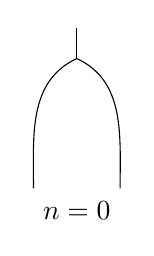
\begin{tikzpicture}[scale=.55]
\draw (1,3.7) to (1,3);

\draw (1,3) to [out=205, in=90] (0,0);
\draw (1,3) to [out=-25, in=90] (2,0);

\node at (1,-.5){$n=0$};
\end{tikzpicture}\hspace*{1cm}
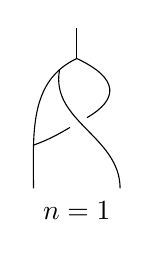
\begin{tikzpicture}[scale=.55]
\draw (1,3.7) to (1,3);

\draw (1,3) to [out=205, in=90] (0,0);

\draw [shorten >= 0cm] (.6,2.73) to [out=-100, in=90] (2,0);

\draw [shorten >= .15cm] (1,3) to [out=-25, in=30, distance=1.1cm] (1,1.5);
\draw [shorten <= .1cm] (1,1.5) to [out=210, in=20] (0,1);

\node at (1,-.5){$n=1$};
\end{tikzpicture}\hspace*{1cm}
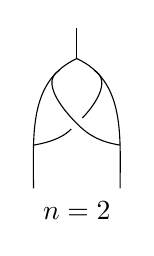
\begin{tikzpicture}[scale=.55]
\draw (1,3.7) to (1,3);

\draw (1,3) to [out=205, in=90] (0,0);
\draw (1,3) to [out=-25, in=90] (2,0);

\draw [shorten >= 0cm] (.6,2.73) to [out=210, in=135] (1,1.5);
\draw [shorten <= 0cm] (1,1.5) to [out=-45, in=170] (2,1);

\draw [shorten >= .1cm] (1.4,2.73) to [out=-30, in=45] (1,1.5);
\draw [shorten <= .1cm] (1,1.5) to [out=-135, in=10] (0,1);

\node at (1,-.5){$n=2$};
\end{tikzpicture}
\end{center}
\end{example}

\item Answer to question in \textbf{Note 6} \par
It is intentional and they have different meanings indeed.

\item Sentences before Examples 6.13 and 6.17 \par
\textit{Replace} notations \textit{with} notation \par
\textit{According to Webster ``notation'' is a ``system'' so in this case it contains two pieces of notation.}

\item Sec. 7 \par
\textit{Add before last paragraph:}
In physics, Gaiotto, Kapustin, Thorngren \cite{gaiotto2016spin, kapustin2017fermionic, bhardwaj2017state} and others have considered cellular decompositions of spacetime together with fields represented by cellular cochains.
In order to express subtle interactions between these fields, they have used cup-$i$ products to define relevant action functionals for topological field theories.
We expect that new topological field theories of interest can be studied using the Steenrod cup-$(p,i)$ products introduced in this work.

\item Acknowledgment \par
\textit{Replace with:}
The authors thank Clemens Berger, Calista Bernard, Greg Brumfiel, Federico Cantero-Mor\'an, Greg Friedman, Kathryn Hess, Jens Kjaer, John Morgan, Andy Putman, Dev Sinha, and Dennis Sullivan for insightful discussions, and the anonymous referee for many keen observations and helpful suggestions.

\item Funding \par
\textit{Replace with:}
A. M. Medina-Mardones acknowledges financial support from Innosuisse grant \mbox{32875.1 IP-ICT-1}.

\item Bibliography \par
\textit{Please replace the corresponding entries:}
\begin{enumerate}
\item
\begin{Verbatim}
@article {adams1957cobar,
	AUTHOR = {Adams, J. F.},
	TITLE = {On the cobar construction},
	JOURNAL = {Proc. Nat. Acad. Sci. U.S.A.},
	FJOURNAL = {Proceedings of the National Academy of Sciences of the United
	States of America},
	VOLUME = {42},
	YEAR = {1956},
	PAGES = {409--412},
	ISSN = {0027-8424},
	MRCLASS = {55.0X},
	MRNUMBER = {79266},
	MRREVIEWER = {W. S. Massey},
	DOI = {10.1073/pnas.42.7.409},
	URL = {https://doi.org/10.1073/pnas.42.7.409},
}
\end{Verbatim}
\item
\begin{Verbatim}
@ARTICLE{medina2021adem,
	author={Brumfiel, Greg and {Medina-Mardones}, Anibal and Morgan, John},
	title={A cochain level proof of Adem relations in the mod 2 Steenrod algebra},
	JOURNAL = {J. Homotopy Relat. Struct.},
	FJOURNAL = {Journal of Homotopy and Related Structures},
	year={2021},
	day={19},
	issn={1512-2891},
	doi={10.1007/s40062-021-00287-3},
	url={https://doi.org/10.1007/s40062-021-00287-3}
}
\end{Verbatim}
\item
\begin{Verbatim}
@ARTICLE{medina2021computer,
	author = {{Medina-Mardones}, Anibal M.},
	title = "{A computer algebra system for the study of commutativity up to coherent homotopies}",
	journal = {arXiv e-prints},
	year = 2021,
	archivePrefix = {arXiv},
	eprint = {2102.07670},
	note = {To appear in Tbilisi Math. J.}
}
\end{Verbatim}

\item
\begin{Verbatim}
@ARTICLE{medina2021cobar,
	author = {{Medina-Mardones}, Anibal M. and {Rivera}, Manuel},
	title = "{The cobar construction as an $E_{\infty}$-bialgebra model of the based loop space}",
	journal = {arXiv e-prints},
	year = 2021,
	archivePrefix = {arXiv},
	eprint = {2108.02790},
}
\end{Verbatim}
\end{enumerate}
\end{enumerate}
\end{document}